\documentclass[
17pt,
  dvipdfmx,
  xcolor={svgnames},
  hyperref={colorlinks,citecolor=DeepPink4,linkcolor=DarkRed,urlcolor=DarkBlue}
  ]{beamer}
\title{A proposal for semantic segmentation model for evaluating Gleason patterns of prostate cancer and integrated diagnostic system using Raspberry Pi}
\author{Ken Enda}
\institute{Department of Cancer Pathology Faculty of Medicine, HOKKAIDO UNIVERSITY}

\usetheme{Berlin}

\usepackage[utf8]{inputenc}
% \usepackage{bxdpx-beamer}
% \usepackage{pxjahyper}
\usepackage{graphicx}
\usepackage{hyperref}
\usepackage{media9}
% \usepackage{movie15}
\usepackage{hyperref}
% \usepackage{parskip}

\newcommand\Fontvi{\fontsize{6}{7.2}\selectfont}

\usepackage[orientation=portrait,size=a0,scale=1.4,debug]{beamerposter}
\usepackage[japanese]{babel}
\usepackage[font=small]{caption}
\usepackage[font=footnotesize]{subcaption}
\setbeamertemplate{navigation symbols}{}

% caption
\addto\captionsjapanese{\renewcommand{\figurename}{Fig}}
\addto\captionsjapanese{\renewcommand{\tablename}{Table}}
\setbeamertemplate{caption}[numbered]

% bin
\renewcommand{\kanjifamilydefault}{\gtdefault}
\setbeamercolor{bibliography item}{fg=black}
\setbeamercolor{bibliography entry author}{fg=black}
% \setbeamercolor{bibliography entry author}{fg=red}
% \setbeamercolor{bibliography entry title}{fg=blue}
% \setbeamercolor{bibliography entry location}{fg=green}
% \setbeamercolor{bibliography entry note}{fg=cyan}

% fig
\makeatletter
\def\@cite#1{\textsuperscript{[#1]}}
\makeatother

\begin{document}
\nocite{*}

\begin{columns}[T]
  \begin{minipage}[]{0.75\columnwidth}
    \vspace{5mm}
    \huge A proposal for semantic segmentation model for evaluating Gleason patterns of prostate cancer and integrated diagnostic system using Raspberry Pi
    \\[5mm]
    \large Ken ENDA \cite{student} \hspace{5mm} Koki ISE\cite{student} \hspace{5mm} Yusuke ISHIDA\cite{teacher} \hspace{5mm} Sinnya TANAKA\cite{teacher}
    {\small
      \begin{thebibliography}{99}
        \beamertemplatetextbibitems
        \setlength{\itemsep}{-.5zw}
        \bibitem{student} Sixth year student, School of Medicine, Hokkaido University
        \bibitem{teacher} Department of Cancer Pathology Faculty of Medicine, Hokkaido University
      \end{thebibliography}
    }

  \end{minipage}

  \begin{minipage}[]{0.08\columnwidth}
    \begin{figure}\centering
      
\includegraphics[width=\columnwidth]{assets/logo_patho2.png}
    \end{figure}
  \end{minipage}

  \begin{minipage}[]{0.08\columnwidth}
    \begin{figure}\centering
      
\includegraphics[width=\columnwidth]{assets/logo_humed.png}
    \end{figure}
  \end{minipage}

  \begin{minipage}[]{0.08\columnwidth}
    \begin{figure}\centering
      
\includegraphics[width=\columnwidth]{assets/logo_hu.png}
    \end{figure}
  \end{minipage}
\end{columns}

\vspace{10mm}

\begin{columns}[T]
  \begin{column}{0.49\columnwidth}
    \begin{block}{\Large Introduction}
      \begin{flushleft}
        In recent years, the development of image analysis technology using deep learning (DL) has been remarkable and research on histopathological imaging has been very successful.  On the other hand, there are few opportunities to actually use the technique and its products in clinical diagnostic practice. Because several steps must be taken to obtain inferential results from DL on histopathological images. For example, to use DL system you may need to take photograph, move the image files to an external storage, walk to physically separated room where DL system places and analyze the images by DL. Because of somthing hassle like them, DL are rarely used directly in clinical practice. \par

\vspace{0.5zh}

In this study, We propose a system that integrate seamlessly microscope and DL system for clinical diagnostics using Raspberry Pi.\par

      \end{flushleft}
    \end{block}

    \begin{block}{\Large Material and method}
      \begin{flushleft}
        First, we created an U-Net\cite{unet} model for semantic segmentation based on images Gleason pattern(GP) of prostate pathological images. The labels are normal glands, GP3, GP4, and GP5. We use VGG16\cite{vgg} for the ecoder part of the U-Net model and nearest sampling for the decoder part.\par

\vspace{0.5zh}

The model was trained by whole slide image of total prostatectomy specimens diagnosed in our department and those labels like Fig\ref{fig:seg_color}. An example output of the model is shown in Fig\ref{fig:dl_sample}. \par

\vspace{-1zh}

\begin{figure}[htbp]\centering
  \begin{tabular}{c}
    \begin{subfigure}[t]{0.20\columnwidth}\centering
      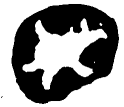
\includegraphics[width=0.7\columnwidth]{assets/gp_pin.png}
      \subcaption{Normal gland:black}
    \end{subfigure}

    \begin{subfigure}[t]{0.15\columnwidth}\centering
      
\includegraphics[width=0.7\columnwidth]{assets/gp_3_2.png}
      \subcaption{GP3:blue}
    \end{subfigure}

    \begin{subfigure}[t]{0.15\columnwidth}\centering
      
\includegraphics[width=0.7\columnwidth]{assets/gp_4.png}
      \subcaption{GP4:green}
    \end{subfigure}

    \begin{subfigure}[t]{0.15\columnwidth}\centering
      
\includegraphics[width=0.7\columnwidth]{assets/gp_5_2.png}
      \subcaption{GP5:red}
    \end{subfigure}

    \begin{subfigure}[t]{0.15\columnwidth}\centering
      
\includegraphics[width=0.7\columnwidth]{assets/gp_3_1.png}
      \subcaption{GP3+4}
    \end{subfigure}

    \begin{subfigure}[t]{0.15\columnwidth}\centering
      
\includegraphics[width=0.7\columnwidth]{assets/gp_5_1.png}
      \subcaption{GP4+5}
    \end{subfigure}
  \end{tabular}
  \label{fig:example}
  \caption{Example of the segmentation}
  \label{fig:seg_color}
\end{figure}

\begin{figure}[htbp]\centering
  \begin{tabular}{c}
    \begin{subfigure}[t]{0.33\columnwidth}\centering
      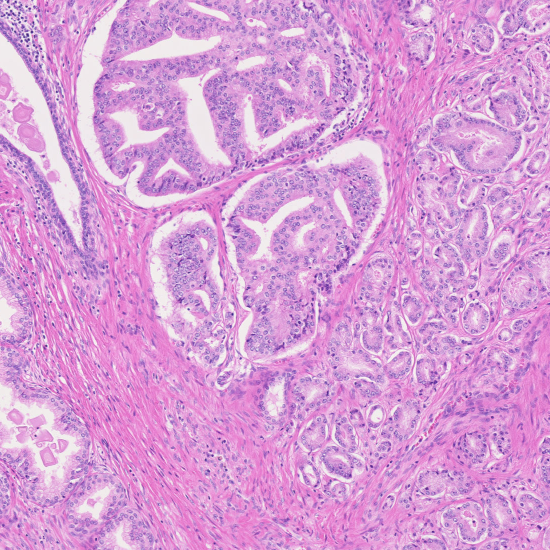
\includegraphics[width=0.9\columnwidth]{assets/ex_org.png}
      \subcaption{Input image}
    \end{subfigure}

    \begin{subfigure}[t]{0.33\columnwidth}\centering
      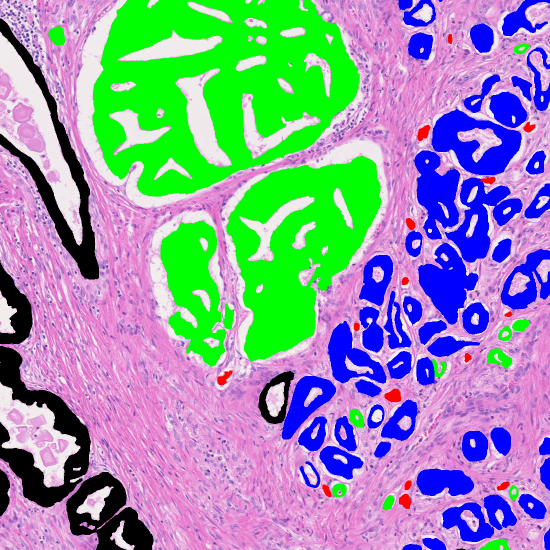
\includegraphics[width=0.9\columnwidth]{assets/ex_gt.png}
      \subcaption{Label image}
    \end{subfigure}

    \begin{subfigure}[t]{0.33\columnwidth}\centering
      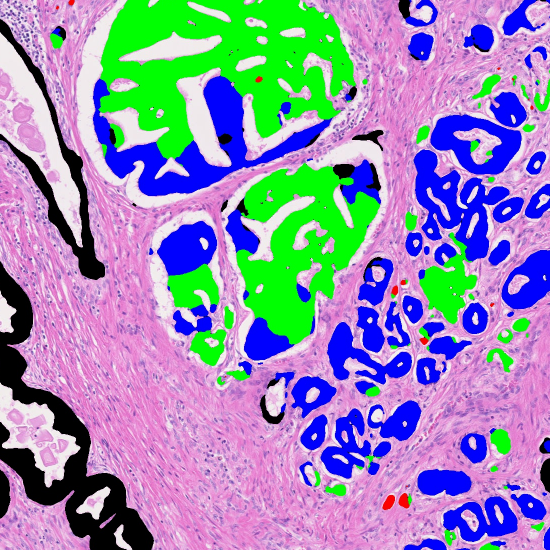
\includegraphics[width=0.9\columnwidth]{assets/ex_pr.png}
      \subcaption{Output image}
    \end{subfigure}
  \end{tabular}
  \label{fig:example}
  \caption{Example output ofr the U-Net model}
  \label{fig:dl_sample}
\end{figure}

The IoU (Intersection over union) calculated by the Jaccard index of the U-Net model were 0.765 for the training datasets and 0.737 for the testing datasets.

\begin{align}
  \label{eq:iou}
  Jaccard\,index = & \; \frac{|PR \cap GT|}{|PR \cup GT|} \\[5mm]
  PR: \mbox{Prediction} & \;\; GT: \mbox{Ground truth} \nonumber
\end{align}

\vspace{0.5zh}

In addition, we developed the client/server applications(Fig\ref{fig:arch}). The client gets the images from the microscopic camera, sends to the server via HTTP and displays the results. It is installed into Raspberry Pi 4 Model B. The server receives the images, passes them to the DL system and serves the results. It is into the computer where DL system works.\par

\vspace{1zh}

\begin{figure}\centering
  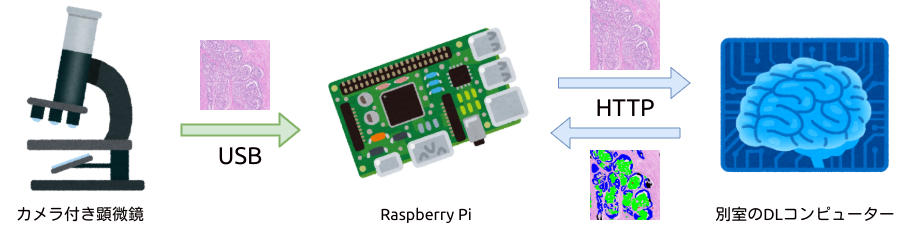
\includegraphics[width=\columnwidth]{assets/arch.png}
  \caption{Architecture of client and server applications}
  \label{fig:arch}
\end{figure}

The DL system and the client/server applications were all written in Python and work on Linux-based computers. Especially the DL system uses PyTorch and the client uses GTK+/GStreamer. The source codes are all available on GitHub.\cite{gh-prostate}\cite{gh-pai} \par

      \end{flushleft}
    \end{block}
  \end{column}

  \begin{column}{0.49\columnwidth}

    \begin{block}{\Large Discussion}
      \begin{flushleft}
        We can get the results of DL analysis in only less than 20 seconds after determining the target area and clicking the analyze button. The effort and hassle of using the DL was reduced to a minimum. However it also means we have to wait 20 seconds. It takes about 10 seconds to analyze 1920×1080 image for the computer with NVIDIA GeForce GTX 1080 Ti and a few seconds to transfer the result image files.

We were faced with the limitations of the Raspberry Pi's performance. Even just playing the video stream transfored from USB-connected microscopic camera, FPS drops. And there was also a delay to alpha composite the result image on the original one. The low performance of the hardware was detracting to the user experience of the client software.

\begin{figure}[t]\centering
  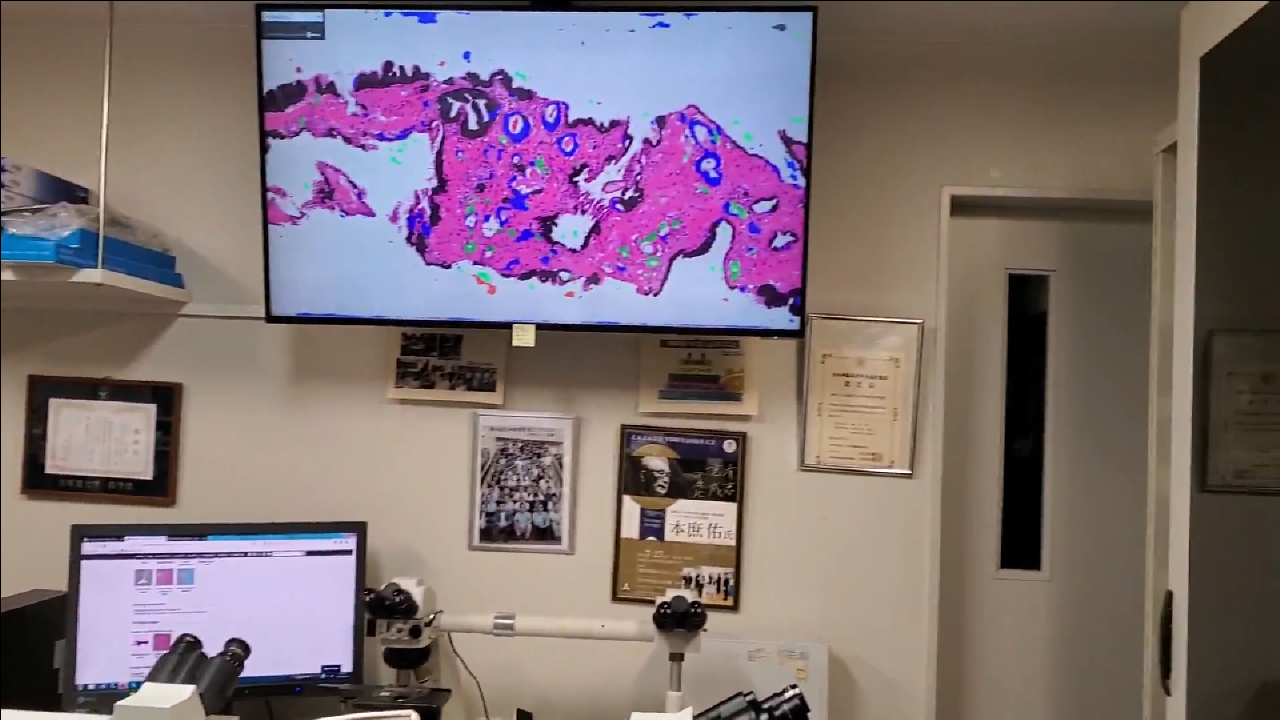
\includegraphics[keepaspectratio]{assets/thumb.png}
  \caption{The client application in action (\href{https://drive.google.com/file/d/16hUGZ2jU2Def9N5ozNaZnLvjnWc-kkNP/view}{Link to the movie})}
  \label{fig:in_action}
\end{figure}

We found they were grateful for the function just to save the image of the view microscopic view without any analytics. Up until now, microscopic camera was connected to display directyl via HDMI.  With the Raspberry Pi in between the camera and the display, we can now take photograph and analyze in addition to usage so far.  Users experienced as if the microscope camera was augmented in functional extension of itself.



      \end{flushleft}
    \end{block}

    \begin{block}{\Large Result}
      \begin{flushleft}
        We discoverd the new side of Raspberry Pi as an extension of the microscope camera itself. Its good point is that it is inexpensive, about 7,000 yen, but the specifications were not sufficient to handle images. We might need a device with another higher performance on this usage.

      \end{flushleft}
    \end{block}

    \begin{block}{\Large References}
      \begin{figure}
        \begin{flushleft}
          \beamertemplatetextbibitems
          \bibliographystyle{junsrt}
          \bibliography{refs}
        \end{flushleft}
      \end{figure}
    \end{block}

  \end{column}

\end{columns}

\end{document}
